%%%%%%%%%%%%%%%%%%%%%%%%%%%%%%%%%%%%%%%%%%%%%%%%%%%%%%%%%%%%%%%%%%%%%%
%%                     delay
%%%%%%%%%%%%%%%%%%%%%%%%%%%%%%%%%%%%%%%%%%%%%%%%%%%%%%%%%%%%%%%%%%%%%%
%\color{blue}
\subsubsection{Glyph: \glyph{delay}}\label{sec:delay}

The glyph \glyph{delay} is used to denote that the \glyph{entity nodes} linked as input does not produce the influence immediately, but a delay after the decision of influencing has been taken.

\begin{glyphDescription}

 \glyphSboTerm SBO:0000225 ! delay.

 \glyphContainer \glyph{Delay} is represented by a circle, with two connectors located at the opposite side for input and output.

  \glyphLabel \glyph{Delay} is identified by the greek letter ``$\tau$`` (``TAU'') placed in an unbordered box attached to the center of the container. 

  \glyphAux \glyph{Delay} does not carry any auxiliary items.

\end{glyphDescription}

\begin{figure}[H]
  \centering
  
\includegraphics[scale = 0.5]{images/delay}
  \caption{The \ER glyph for \glyph{delay}.}
  \label{fig:delay}
\end{figure}

\begin{figure}[H]
  \centering
  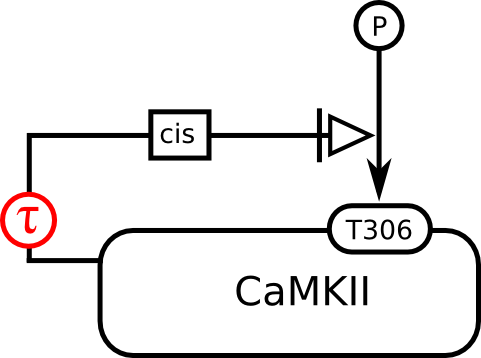
\includegraphics[scale = 0.5]{examples/ex-delay}
  \caption{Example of the \glyph{delay} logical operator, showing that the stimulation of the phosphorylation of CaMKII on threonin 306 takes place a measurable amount of time after the decision of stimulation is triggered.}
  \label{fig:ex-delay}
\end{figure}

%\normalcolor
